\section{Assessing Aesthetic Criteria} \label{p2approach}

\begin{figure}
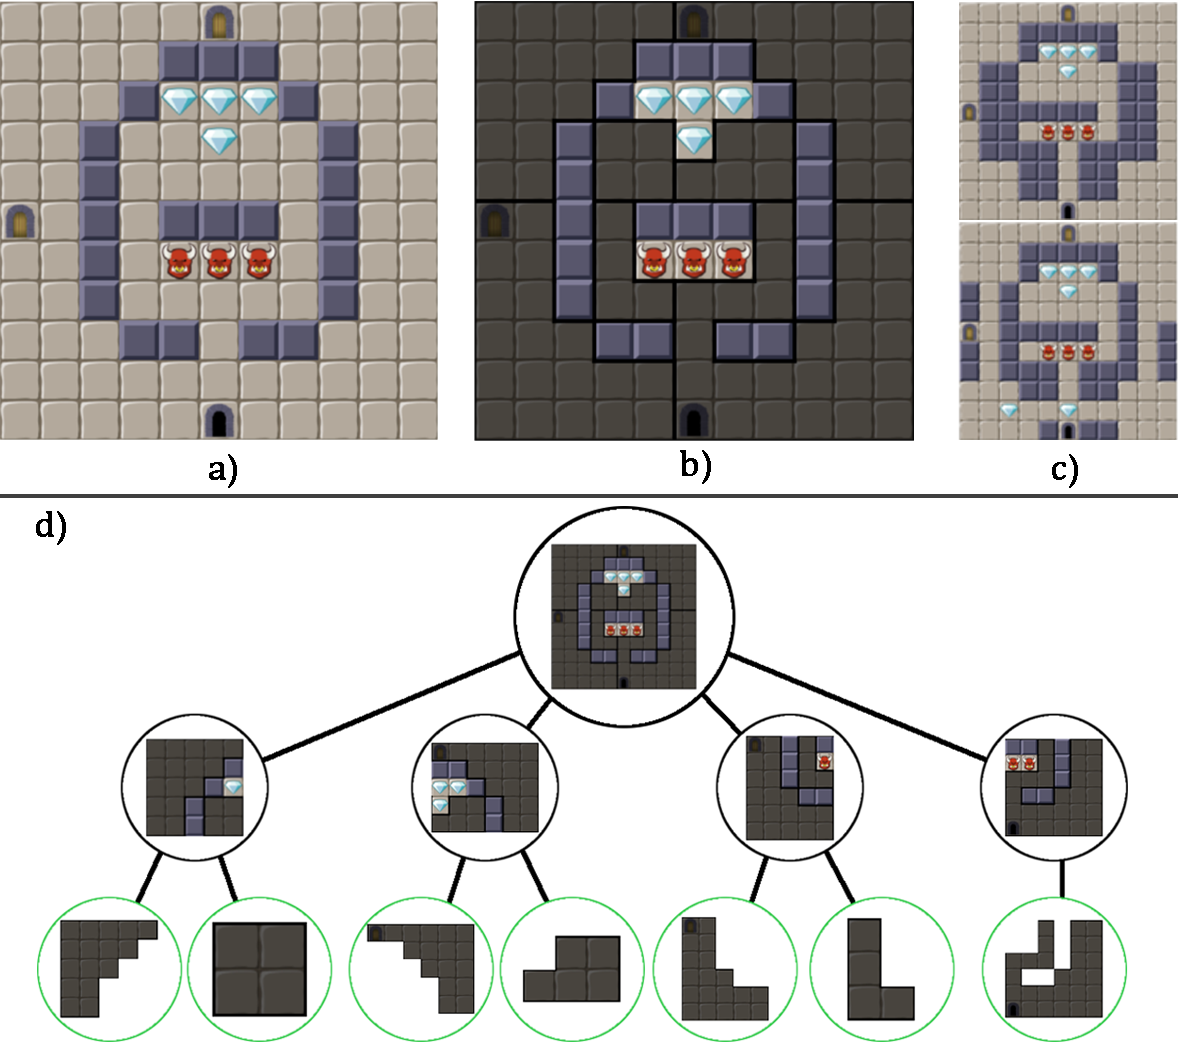
\includegraphics[scale=0.2]{Figures/map-representation-figure-test}
\caption{A sample edited room (a) with its division into zones (b) based on the tiles locked by the user. Suggestions preserve these locked tiles (c). The room and its zones are internally represented with a tree structure (d), where the leaf nodes (green) are the valid candidates to operate within an individual.}
\label{p2fig:map-representation}
\end{figure}

Our approach is divided in two; on one side, the algorithm implicitly has control over different aesthetic criteria using the edited room as a base to measure symmetry and similarity for the EA. On the other side, the designer was given control over what they wanted to preserve by being able to select tiles in the room to be immutable (i.e. not changeable in following generations).

\subsection{Preserving Custom Aesthetic Structures}

%To preserve the aesthetic criteria of a designer's edited room, we give him/her the ability to manually lock custom structures in it, preserving these in the upcoming the next suggestions. This is possible by incorporating a new brush which is used as a complementary modifier when editing the room. The designer can now lock any range of tiles, making it possible to preserve individual tiles, shapes, patterns, routes and even design patterns as shown in Figure \ref{p2fig:possible-zones}. 
To preserve the aesthetic criteria of a designer's edited room, we give the users the ability to manually lock custom structures in it, preserving these in the upcoming suggestions. This is possible by incorporating a new brush which is used as a complementary modifier when editing the room. The designer can now lock any range of tiles, making it possible to preserve individual tiles, shapes, patterns, routes and even design patterns as shown in Figure~\ref{p2fig:possible-zones}.

The process to subdivide the room is straightforward; the designer is presented with the room to be edited, and by using the lock brush, the room seamlessly subdivides and creates zones, which classifies the room's tiles into two sets: the immutable tiles (i.e. invalid or locked) and the mutable tiles (i.e. valid or unlocked).

An individual's genotype is now changed from a direct encoding (each tile is a gene) to a semi-direct encoding using a tree structure, with the nodes of the tree as different zones of the room, constructed from the mutable and immutable tiles, and the leaf nodes, only containing sets of mutable tiles, as candidates to be used for crossing and mutation. Figure~\ref{p2fig:map-representation} shows the room, it's division into zones and the tree representation used by the EA. 

The advantages of this representation are that it allows the EA to reduce the search space by only considering valid zones of the room, and improves the crossover operator by allowing the exchange of irregular shapes between individuals along different parts of the room.

%An individual's genotype is now changed from a direct encoding (each tile is a gene) to a semi-direct encoding using a tree structure, with the nodes of the tree as different sections of the room and the leaf nodes as candidates to be used for crossing and mutation. Figure~\ref{p2fig:map-representation} shows the room, it's division into zones and the tree representation used by the EA. This change in the individual representation improves the crossover operator by allowing the exchange of irregular shapes between individuals along different parts of the room. This results in an increased presence of custom (user-shaped) building blocks among the generated offspring.

In practice, this solution allows users to preserve any aesthetic change (either significant or detailed) that they want to keep in further generations, while still receiving novel suggestions created following the pattern-based fitness function. It also means that the construction of the dungeon can be performed differently: instead of manually editing a room first to later generate appealing solutions based on it, the user can now start from a suggestion, selecting parts of it that look promising that are kept through subsequent generations, until the user's needs and criteria are met.

%In practice, this solution allows users to preserve any aesthetic change (either significant or detailed) that they want to keep in further generations, while still receiving novel suggestions created following the pattern-based fitness function. It also means that the construction of the dungeon can be performed differently: instead of manually editing a room first to later generate appealing solutions based on it, the user can now start from a suggestion, selecting parts of it that look promising that are kept through the following generations of procedurally generated suggestions, until the user's needs and criteria are met.

%In practice, this solution allows users to preserve any aesthetic change (either significant or detailed) that they want to keep in further generations, while still receiving novel suggestions created following the pattern-based fitness function. It also means that the construction of the dungeon can be performed differently: instead of manually editing a room first to later generate appealing solutions based on it, the user can now start from a suggestion, selecting parts of it that look promising that are kept through the following generations of procedurally generated suggestions, until one meets his/her needs and criteria.

\subsection{Evaluating Symmetry and Similarity}

\begin{figure}
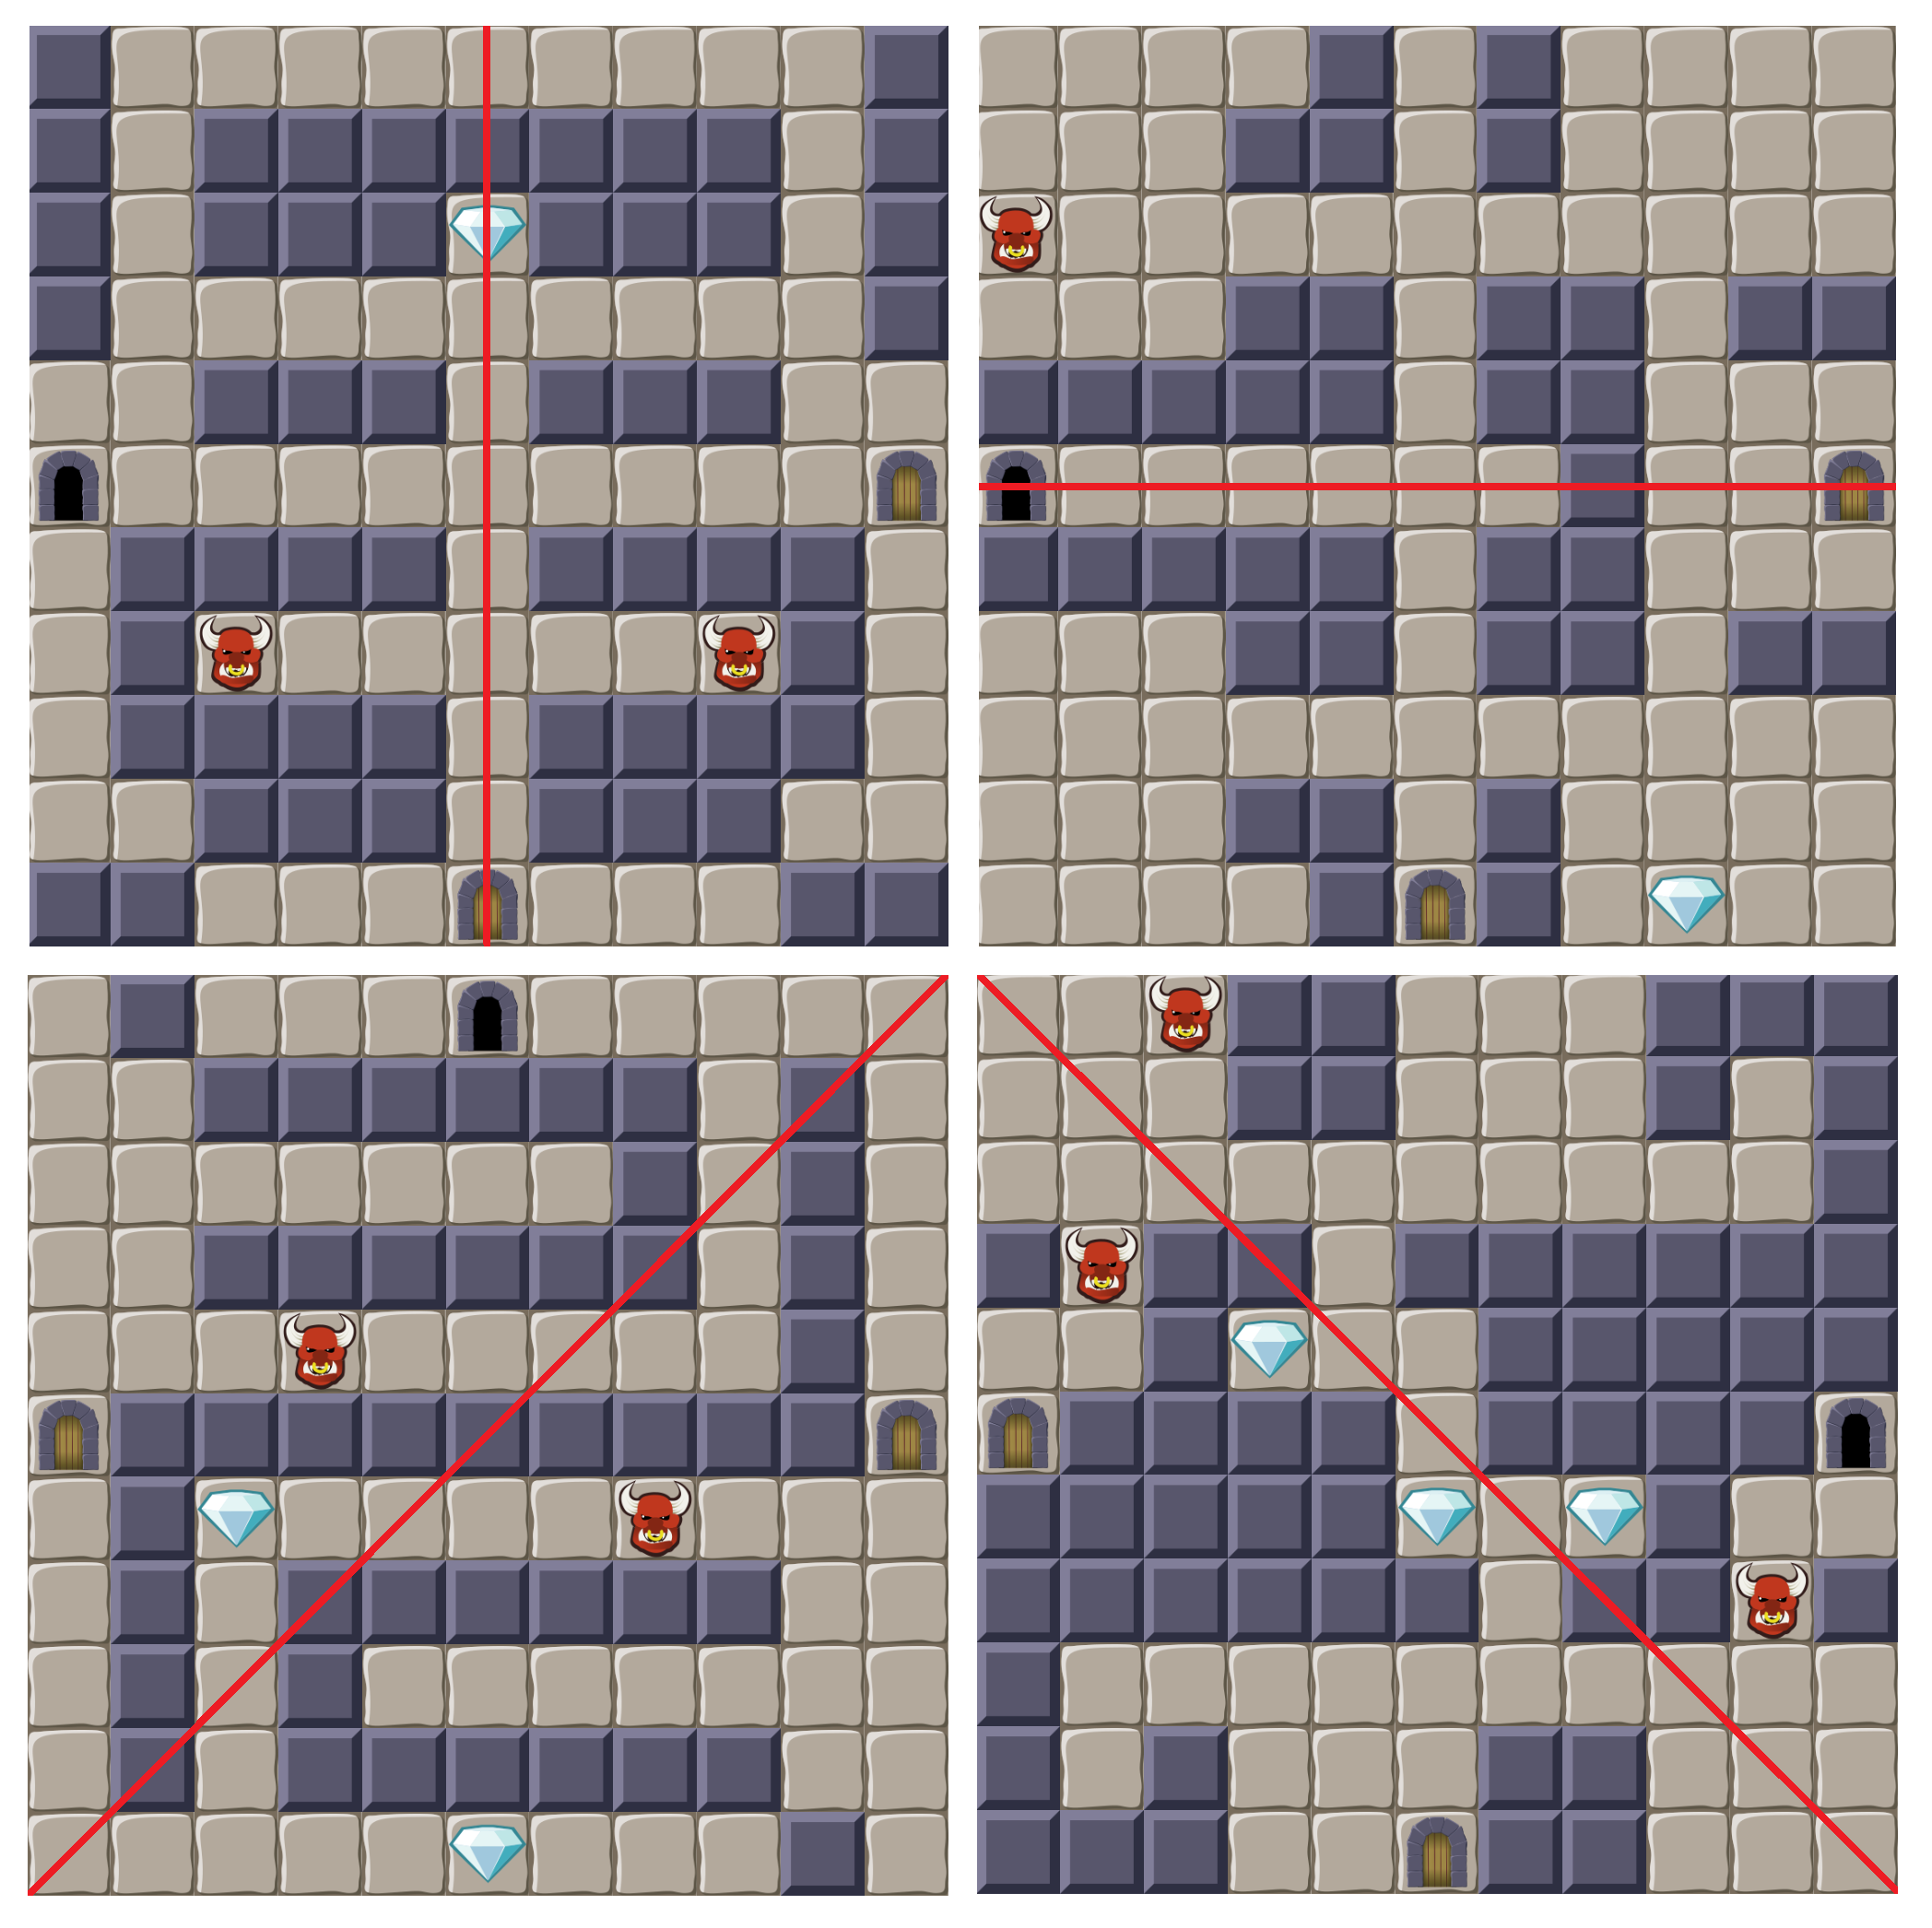
\includegraphics[scale=0.09]{Figures/DifferentSymmetry}
\caption{Different types of symmetry evaluated}
\label{p2fig:symmetry-types}
\end{figure}

While the pattern-based fitness function worked well for functionality purposes, it did not consider nor capture any aesthetic aspects into it. Therefore, in order to consider and preserve visual aesthetic criteria, we evaluate the rooms for their symmetry  along the X and Y axes, backslash and front slash diagonal as shown in Figure \ref{p2fig:symmetry-types} and calculate the similarity that subsequent individuals had in comparison with the original edited room. For simplicity, we differentiate the room by impassable (i.e. walls) and passable (i.e. floor, treasure and enemy) tiles.

%In order to implicitly consider and preserve visual aesthetics criteria, we evaluate the rooms for their symmetry  along the X and Y axes, backslash and front slash diagonal as shown in Figure \ref{p2fig:symmetry-types} and calculate the similarity that subsequent individuals had in comparison with the original edited room. For simplicity, we differentiate the room by impassable (i.e. walls) and passable (i.e. floor, treasure and enemy) tiles.

%In order to implicitly consider and preserve visual aesthetics criteria, we evaluated the rooms for their symmetry  along the X and Y axes, backslash and front slash diagonal as shown in Figure \ref{p2fig:symmetry-types} and calculated the similarity that subsequent individuals had regarding the original edited room. For simplicity, we differentiated the room by unpassable (i.e. walls) and passable (i.e. floor, treasure and enemy) tiles.

\subsubsection{Symmetry evaluation}

%unpassable
%To calculate the symmetry of a room we evaluate the impassable tiles of one side against their corresponding tile on the other side for the X and Y axes and diagonals. The highest symmetric value is then used to calculate a curve ranging from 0 to 1, using equation \ref{p2eq:Symmetry}.

To calculate the symmetry of a room we evaluate the impassable tiles of one side against their corresponding tile on the other side for the X and Y axes and diagonals. The highest symmetric value is then used in equation~\ref{p2eq:Symmetry} to calculate the fitness.

\begin{equation} \label{p2eq:Symmetry}
f_{symmetry} = \frac{highestSymmetricValue} {totalWalls}
\end{equation}

Equation~\ref{p2eq:Symmetry} allow us to calculate symmetry while also preventing the favoring of more walls. Once calculated, we weight the result into the individual's fitness, and as consequence it would favor more or less symmetric rooms and preserve the room's configuration as it can be seen in Figure~\ref{p2fig:symmetry-result}.

\begin{figure}
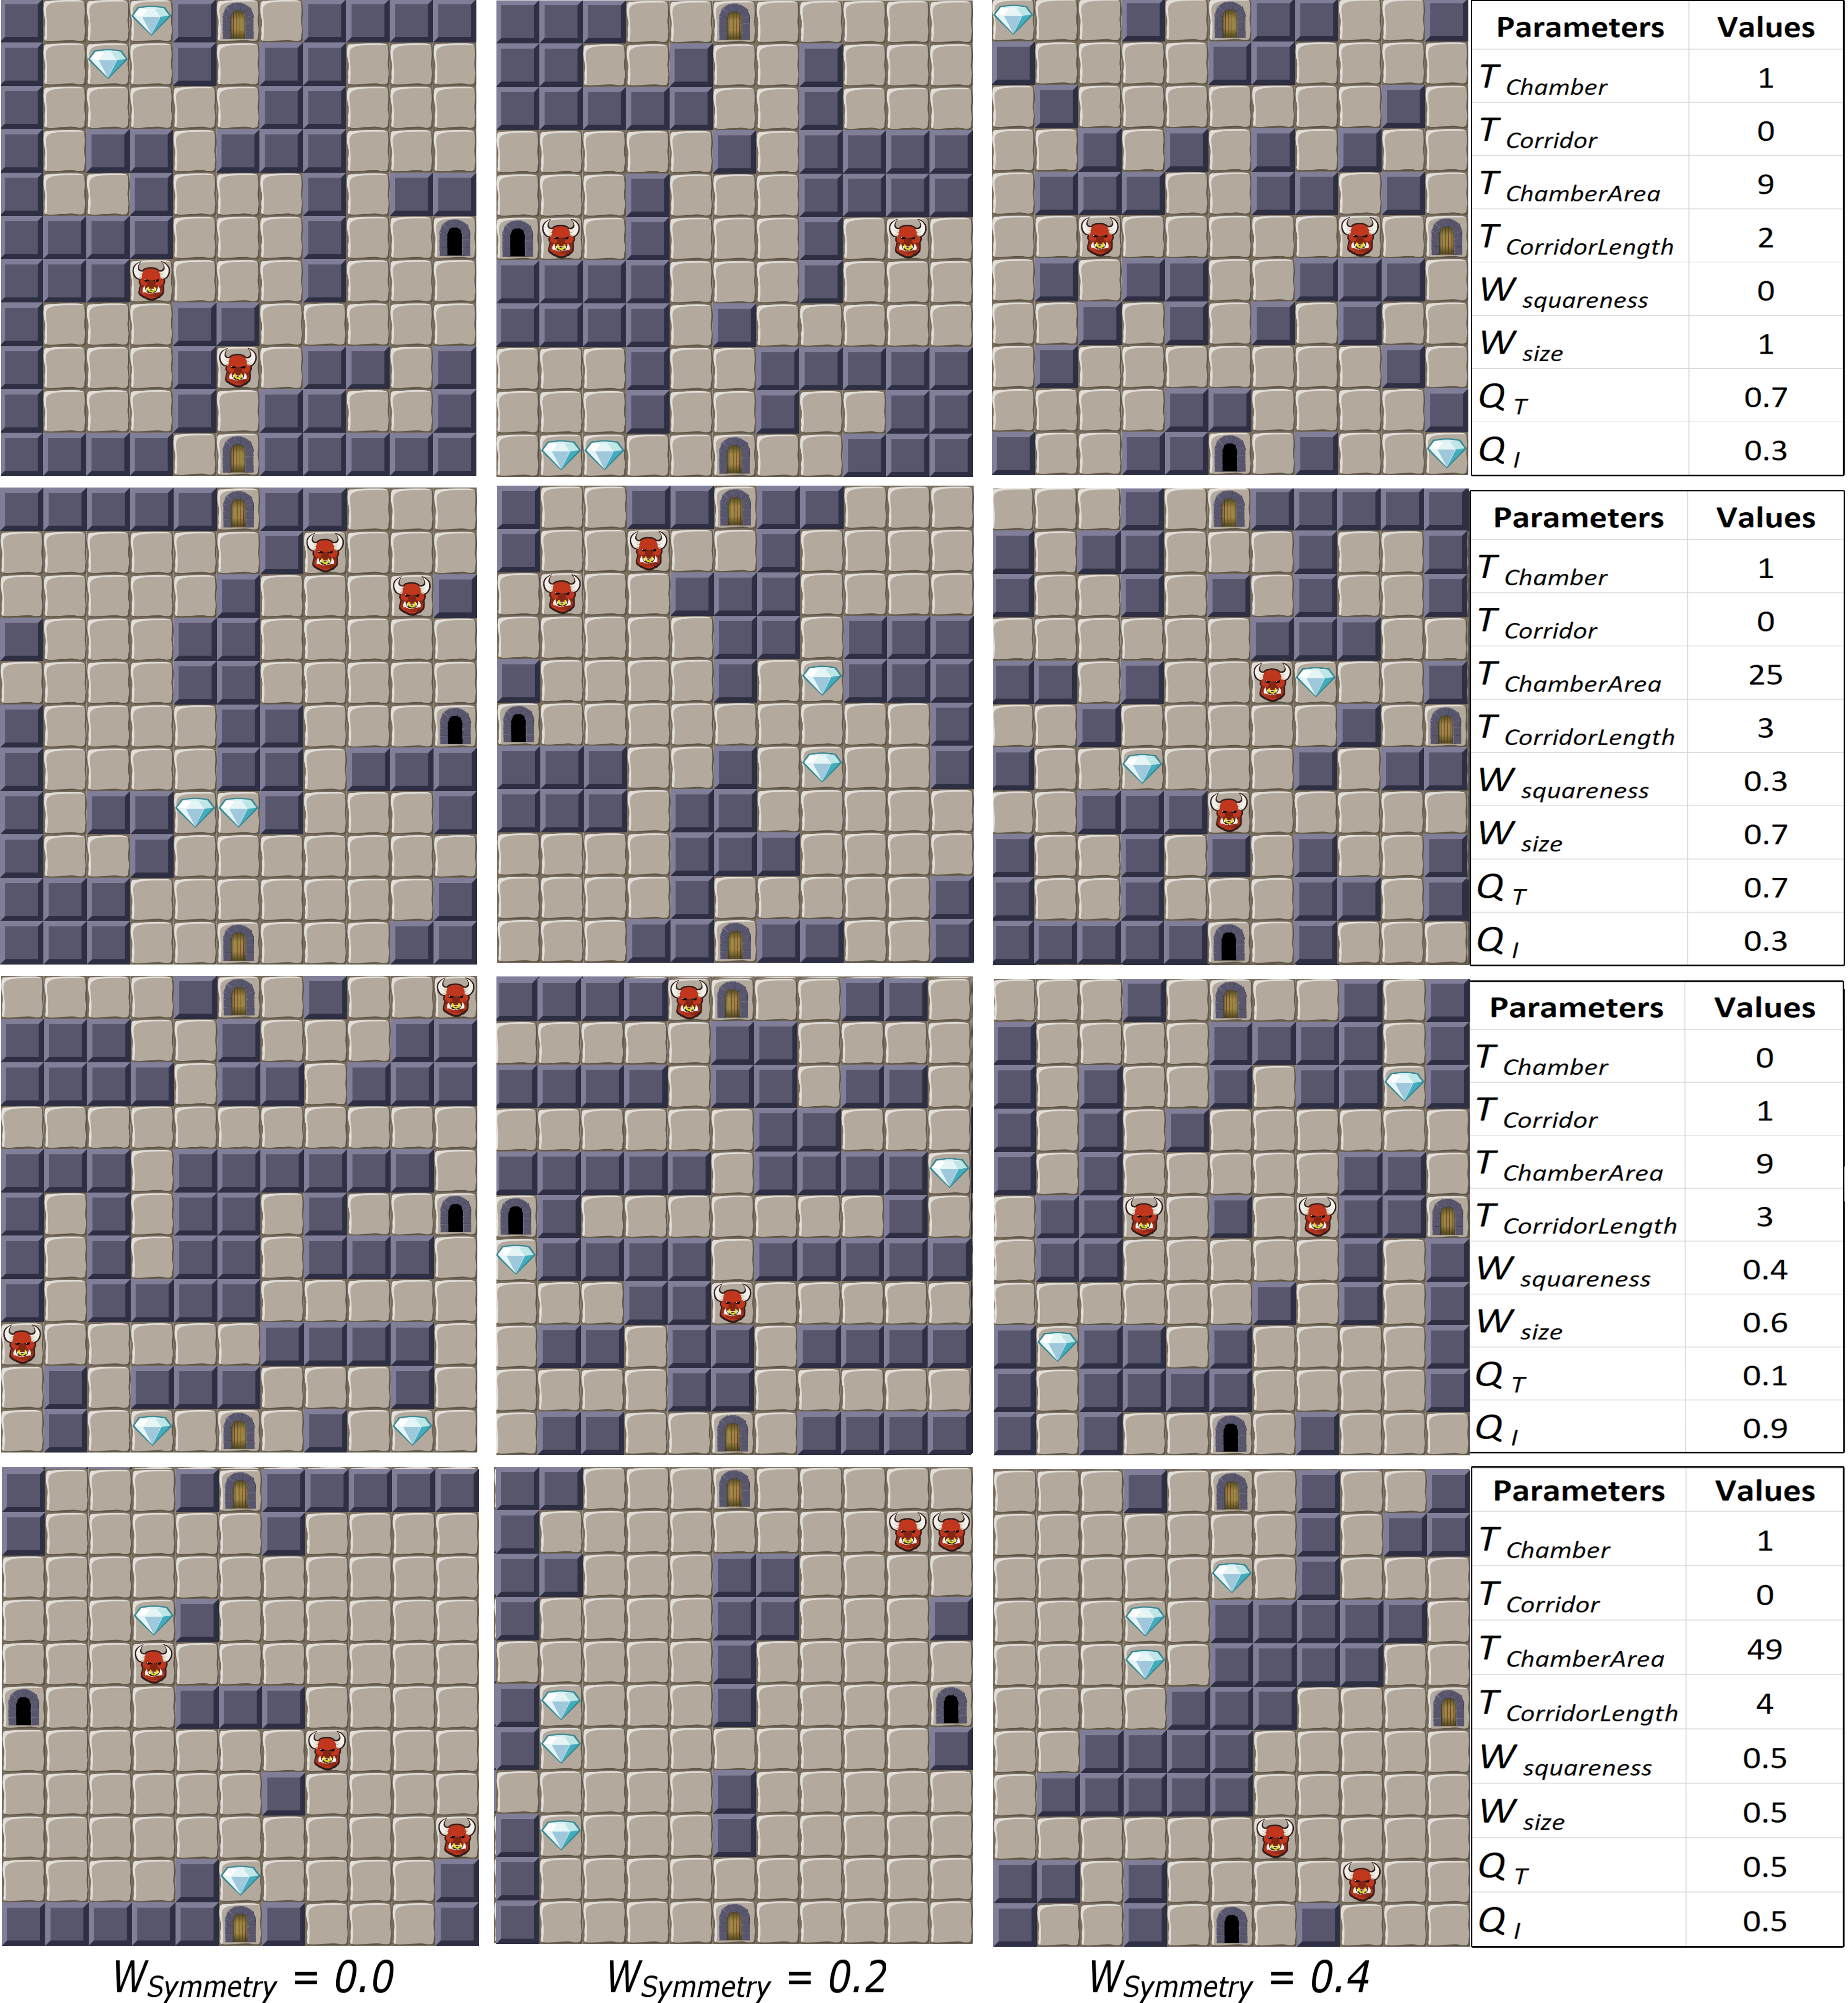
\includegraphics[scale=0.082]{Figures/symmetry-result-figuer}
\caption{Each row shows three results (\(W_{symmetry}=0, W_{symmetry}=0.2, W_{symmetry}=0.4\) ) produced under the settings displayed on the rightmost column. Metrics adapted from \cite{Baldwin2017Mixed-initiativePatterns}.}
\label{p2fig:symmetry-result}
\end{figure}

\subsubsection{Similarity evaluation}

The similarity value between an edited room and successive evolved rooms is calculated by comparing every tile in the original with the corresponding tile in subsequent individuals. Once the total amount of equal tiles is known, we calculate the similarity percentage based on the total amount of tiles, following equation~\ref{p2eq:ProcentSimilar}. 

\begin{equation} \label{p2eq:ProcentSimilar}
similarityPercentage = \frac{totalTiles - notSimilarTiles} {totalTiles}
\end{equation}

%In order for the similarity percentage to be useful we introduced \(idealSimilarityPercentage\) as a parameter related to how similar we want the individuals to be, and use it to normalize the final \(f_{similarity}\) as shown in equation~\ref{p2eq:FSimilarity} or if \(SimilarityPercentage\) was higher then we use~\ref{p2eq:FSimilarity2}.

%\begin{equation} \label{p2eq:FSimilarity}
%f_{similarity} = \frac{SimilarityPercentage} {idealSimilarityPercentage}
%\end{equation}

%\begin{equation} \label{p2eq:FSimilarity2}
%f_{similarity} = \frac{1 - SimilarityPercentage} {1 - idealSimilarityPercentage}
%\end{equation}

We introduced a second parameter called \(idealSimilarity\), which represents how similar we want the individuals to be. Following equation~\ref{p2eq:FSimilarity} we measured the error between both similarities and used it as the similarity fitness. 

\begin{equation} \label{p2eq:FSimilarity}
f_{similarity} = 1 - \left |idealSimilarity - SimilarityPercentage \right |
\end{equation}

The result of incorporating the similarity evaluation into the final fitness is shown in Figure~\ref{p2fig:similarity-result} where is observable that depending on the \(idealSimilarityPercentage\) the original room goes from having a slight variation to start losing its resemblance.

\begin{figure}
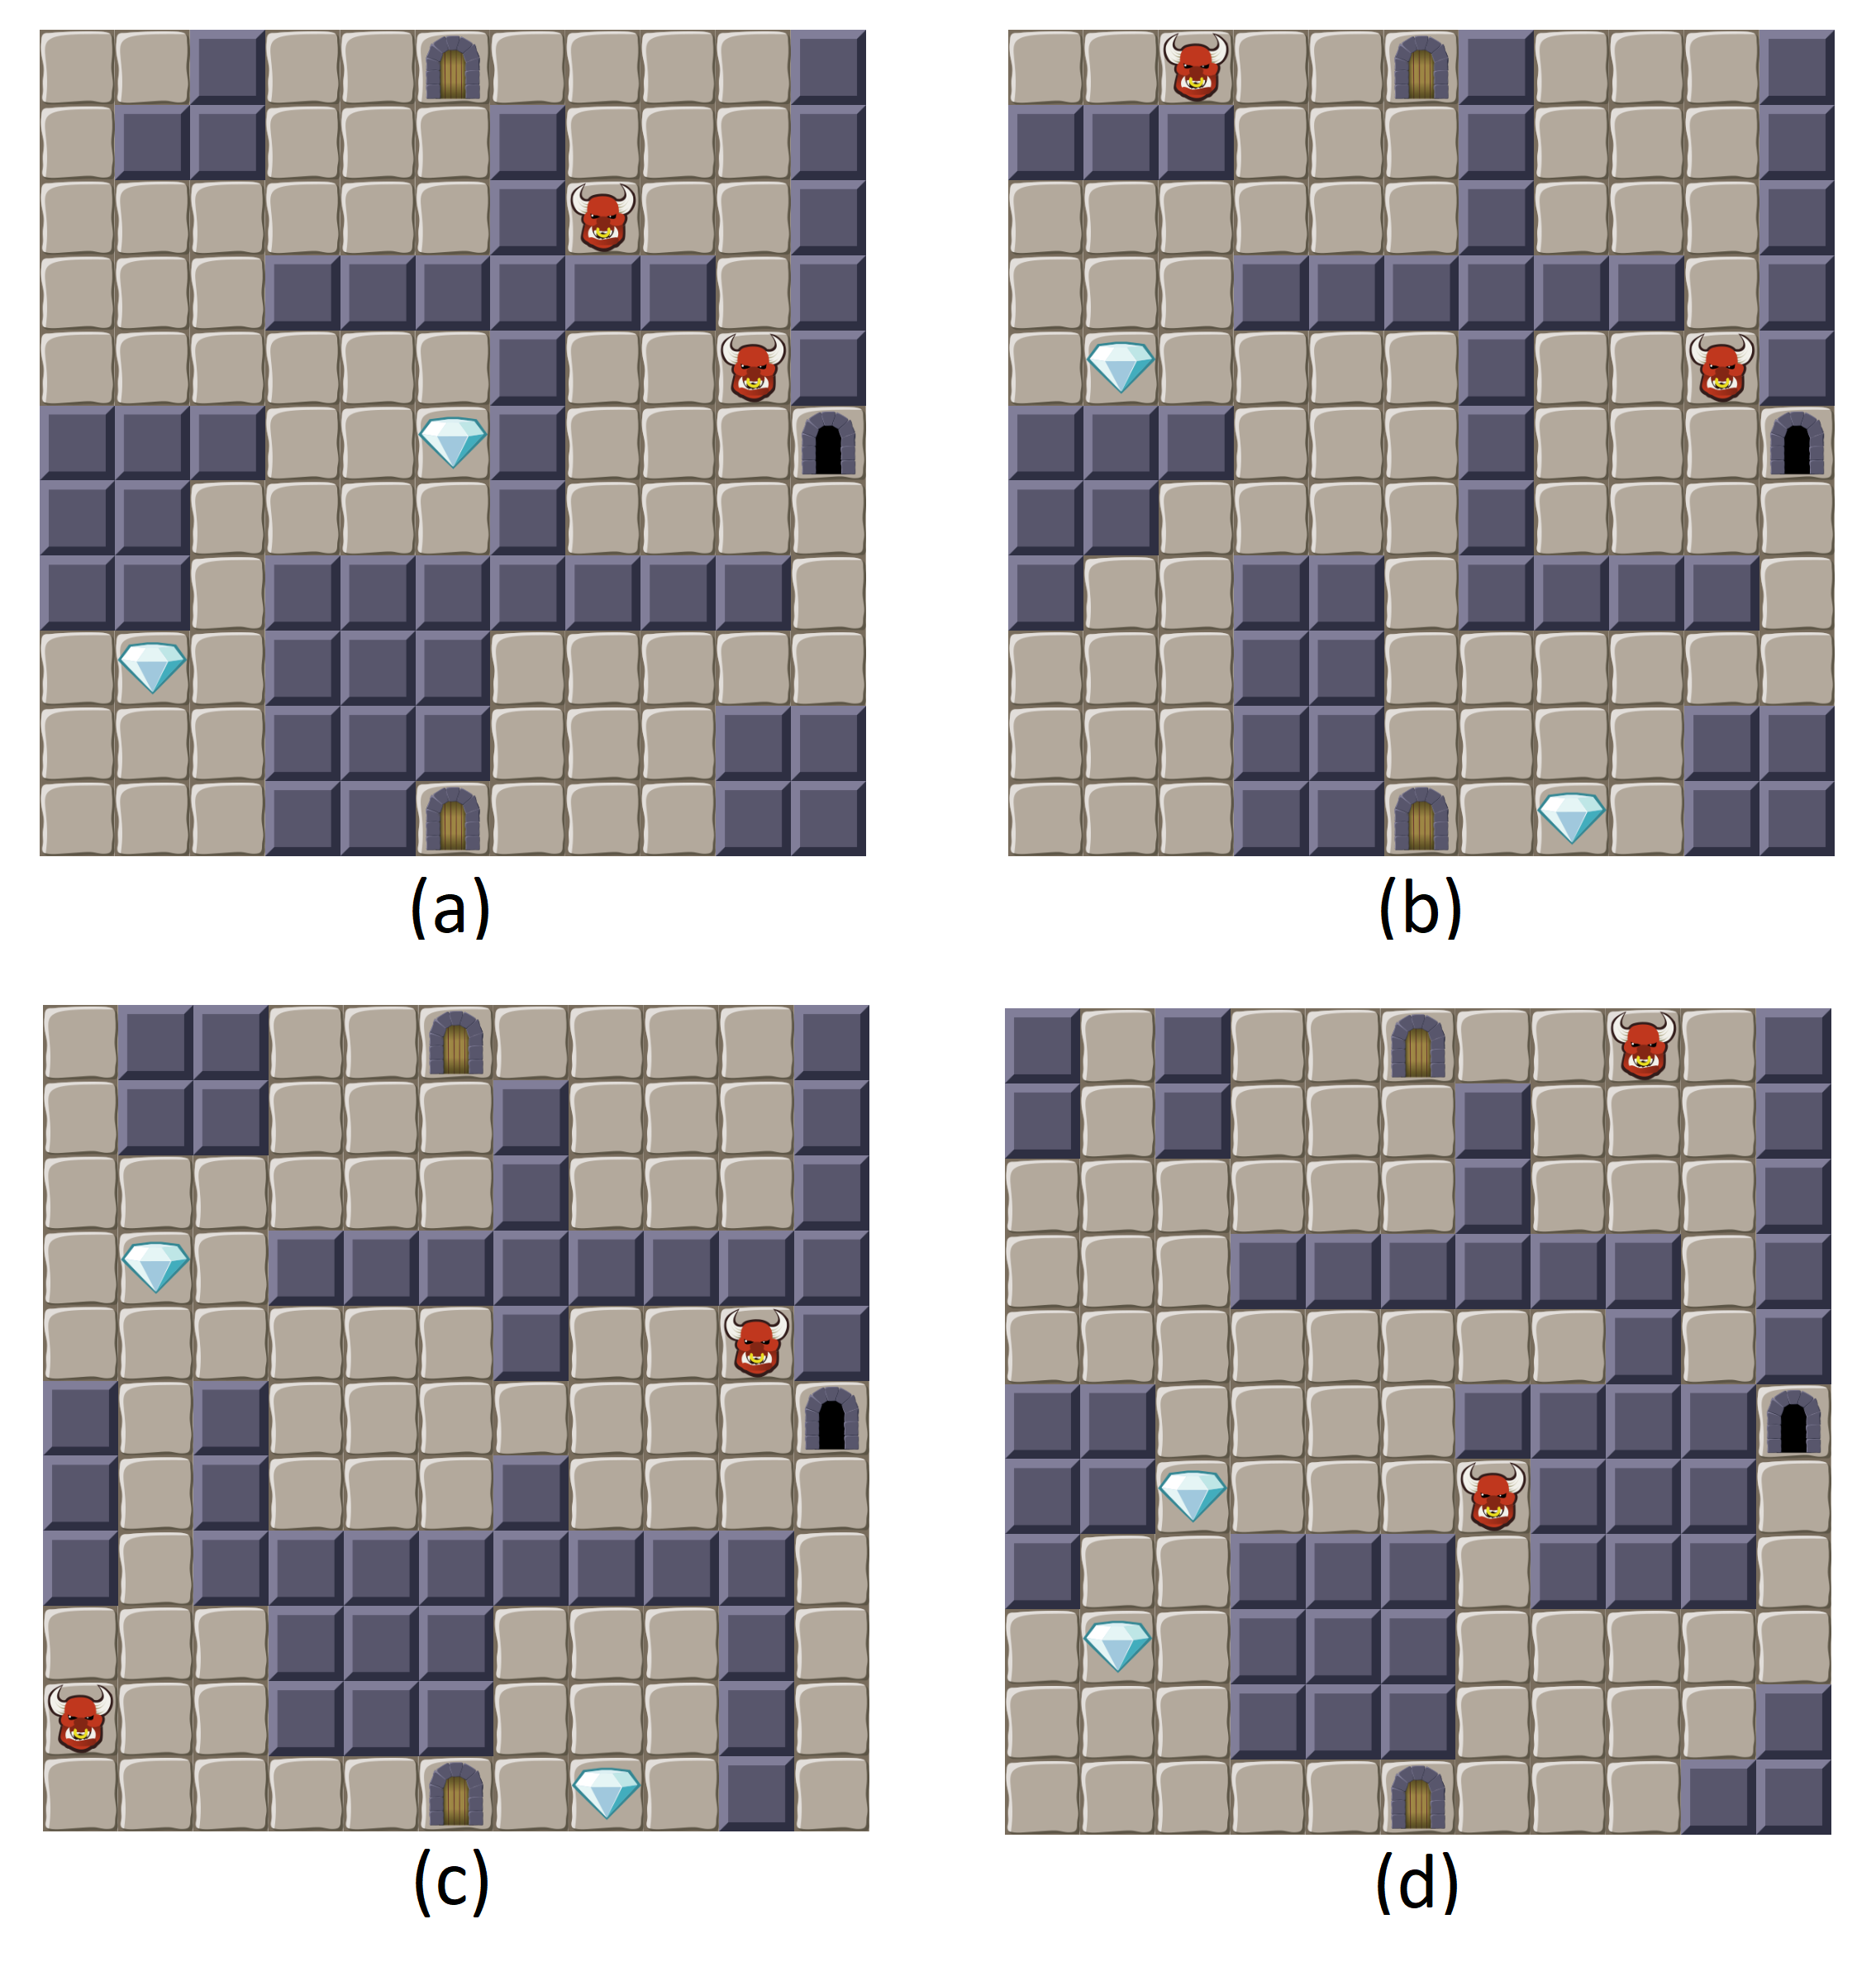
\includegraphics[scale=0.082]{Figures/figure-similarity}
\caption{(a) Sample original room and the evolved solutions with different \(idealSimilarity\) values in order: (b)~0.95, (c) 0.90 and (d) 0.85.}
\label{p2fig:similarity-result}
\end{figure}

Finally and expanding over the previous work on EDD~\cite{Baldwin2017TowardsGeneration}, these calculations (i.e. \(f_{symmetry}\) and \(f_{similarity}\)) are included into the existing fitness evaluation of an individual as shown in equation \ref{p2eq:SiSyFitness}. \(f_{inventorial}\) and \(f_{spacial}\), evaluates the overall layout of the room, and the frequency and quality of the design patterns in the room, respectively. An in-depth explanation of both can be found in~\cite{Baldwin2017TowardsGeneration}.

%Finally and expanding over the previous work on EDD~\cite{Baldwin2017TowardsGeneration}, these calculations are included into the existing fitness evaluation of an individual as shown in equation \ref{p2eq:SiSyFitness}.

\begin{equation} \label{p2eq:SiSyFitness}
\begin{split}
f_{fitness}(r) & = (\frac{a}{10}f_{inventorial}(r) \,+ \, \frac{b}{10}f_{spacial}(r) \\ 
 & \, + \; \frac{c}{10}f_{symmetry}(r)) \ * \ f_{similarity}(r)
\end{split}
\end{equation}